\documentclass{article}
\usepackage{graphicx}
\usepackage{a4, fullpage}
\usepackage{bibtopic}
\usepackage{float}
\usepackage{amssymb,amsmath}
\usepackage[T1]{fontenc}
\usepackage{graphicx}
\usepackage{multicol}
\usepackage{alltt}
\begin{document}

%-------------------------------------------------------------------------------
%    TITLE PAGE
%-------------------------------------------------------------------------------

\begin{titlepage}
\newcommand{\HRule}{\rule{\linewidth}{0.5mm}}
\center
\textsc{\LARGE Imperial College London}  \\[1.5cm]
\textsc{\Large Department of Computing}  \\[0.5cm]
\textsc{\large Course 350: Management and Business for Computing Engineers} \\[0.5cm]

\HRule \\[0.6cm]
{\huge \bfseries name of company here} \\[0.3cm]
\HRule \\[1.5cm]

\begin{minipage}{0.4\textwidth}

% author
\begin{flushleft} \large \emph{Authors:} \\
Alina     \textsc{Boghiu}    \\
Giovanni  \textsc{Charles}   \\
Adam      \textsc{Fiksen}    \\
Sahil     \textsc{Jain}      \\
\L ukasz  \textsc{Koprowski} \\
Rutwik    \textsc{Shah}      \\
John      \textsc{Walker}    \\
\end{flushleft}

% supervisors
\end{minipage}~
\begin{minipage}{0.4\textwidth}

\begin{flushright} \large \emph{Lecturer:} \\
Nick \textsc{Coutts}
\end{flushright}


\end{minipage}\\[4cm]

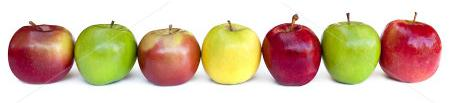
\includegraphics[width=\textwidth]{apples.jpg}

\end{titlepage}

%-------------------------------------------------------------------------------
\tableofcontents
\newpage

\section{Executive summary}

business model = product (disguised as service for legal reasons - absolut?)

business objective 
maximise sales 
 - new to the market
   explain the required infrastructure to sell a lot 

\newpage

\section{Vision statement}

Our mission is to bring a mid priced cider to the people of India. India
has the second largest population in the world, and has an estimated market size
of 500 million alcohol consumers [better estimate]. At the moment, there is one 
provider of cider in India, and we would like the change that.

We want to be a brewery. We will brew our own cider in the state of Himachal
Pradesh, which is the source of the majority of the apples in India. Along with
producing cider, we will sponsor other exclusive bars and clubs.

Operating in India which is well known for its corruption, we want to practice
ethical development. eg corrupt free, no bribes, no blood cider forced labour
fairtrade

We hope to gain popularity in major establishments, in Delhi and Mumbai through 
the open minded youth and bar owners.

Our cider will become a desired commodity through exclusivity and we will be
able to research our market further at this point with minimal risk.

We will adapt and pick up popularity and scale up to make it available to the
public. 

%please discuss even if you do not think it is an issue
Operating in India which is well known for its corruption, we want to practice
ethical development. eg corrupt free, no bribes, no blood cider forced labour
fairtrade

ethics.
fairtrade - look at poverty + with partners
poverty - provide jobs and food to the villagers. improve infrastructure (added benefits - tax exemptions) 
religion - no issue, alcohol is still sold across all of india 
corruption - no bribes, do everything by the books 
age restriction - different restrictions for different states, alcohol content 
health - people already drink, we arent trying to get more people to drink, just introduce it to current drinkers
eco(water recycling, using up all the apples) - recycle apple waste. recycle all water. solar energy. supply of apples
%add as you please

type = pvt. ltd. co. - control of the company
\newpage
\section{Management team}
\newpage
\section{Introduction to the market}
\newpage
\section{Products and services offered}
\newpage
\section{Marketing plan}

\subsection{Route to Market}
Our proposed route to market begins with the launch of a microbrewery in [city].
This is in order to test manufacture on a small scale and conduct market research for later expansion. 

[Explaination of our brewpub]
\subsubsection{Be At One}
B@1 was founded from the ashes of an indian restaurant in Battersea park by
three experienced bartenders.

They started their bar on £60,000 raised from savings and car loans and after a
year grew to a stage where they could start a second bar.

We believe their success stems from their intimate knowledge of the local drinkers and thier personal service to create a great night for each customer.

\subsubsection{Red Bull}
Dietrich Mateschitz attempted to introduce an existing Thai drink, a favourite
for local truck drivers, to a western market, an objective which
mirrors our own.

After initial market research he was strongly advised not to continue with his
venture. He continued regardless on the grounds that the research would be
relevant for an existing product but not his new 'energy drink' which was
unheard of at the time.

He then employed a focused, marketing intensive business strategy for his new product. We believe that this was important in getting people to warm to the new unfamiliar product, and retain its strong market position despite the emerging competitors. 

\subsubsection{}

\subsection{Market Analysis}
\subsubsection{Current Competitors in the Cider Market}
At the moment, there is only one company which produces cider in India.
The company, Green Valley Cider, produces Tempest Cider in the state of Himachal
Pradesh, where they own several acres of apple orchards.

\subsubsection{Current Competitors in the Microbrewery Market}
\begin{itemize}
\item Rockman's Beer Island, Gurgaon - Located in the largest shopping mall in 
			 Gurgaon (bordering New Delhi), Rockman's Beer Island was India's first
			 micro pub brewery. They offer four types of beer: Lager Strong Beer, Dark
			 Beer, Lager Beer and Wheat Beer, and they aim to serve some exclusive
 	     flavoured beers by the summer. Along with the micro pub brewery, they also
			 own an exclusive German restaurant and a digital auditorium covering an
	     area of around 3500 m$^2$. Rockman's are planning to expand now by opening
			 their branch in different locations in India.
\item Toit, Bangalore - Located in the Technology capital of India, Toit has been
			 doing really well since it has opened. They offer 6 different types of beers,
			 which are Toit's Basmati Blonde, Tintin Toit, Toit Weiss, Toit Red, Colonial
			 Toit and Toit's Dark Knight. They are currently in the process of introducing
			 exclusive Toit merchandise, along with their wide selection of food and alcohol.
			 Toit are planning on making the branch national by the end of this year.
\item The Biere Club, Bangalore - Another micro pub brewery which is located in
			 Bangalore, The Biere Club also brews around 6 different types of beers, which
			 include Lager, Ale and Wheat. The Biere Club are planning on making
			 partnerships with rich individuals for expansion in the future.
\item Doolally, Pune - Located in Pune, Doolally has been operational for around
			 three years. It is located in a boutique hotel, and plans to open in a few more
			 locations soon.
\end{itemize}

\subsubsection{Conclusion}
As we can see, there is a large market for alcohol in India, who are eager to try
out new things, which can be seen by the successes of these microbreweries. As India
continues to grow to become a bigger powerhouse in the world, it will attract more
foreigners, which means that people who already know about cider and like it
will increase in the country. This increasing market size makes us believe that
cider will become increasingly popular in India once introduced properly.

\subsection{Advertising}
\subsubsection{Current Laws Affection Alcohol Advertising}
In the 90s, extensive surveys resulted in the conclusion that liquor advertisements
were directly influencing the consumer's purchasing behaviour, which led to the 
introduction to new laws. Ever since the Cable Television Network Amendment Bill 
came into effect on September 8$^{th}$ 2000, advertising alcoholic beverages on 
television networks and billboards is completely banned in India. 

\subsubsection{Surrogate Advertisement}
Although illegal, alcohol companies have found a way to spread their name through
the media by the use of surrogate advertisment. Surrogate Advertisement refers
to the form of advertisement which is used to promote banned producted, which is
alcohol in our case, in the disguise of another product. 
Nearly all alcohol brands have now created other products which they use to advertise
their alcohol. Examples of this include Bagpiper Whiskey creating a Club Soda with
their brand name, Royal Stag creating Music CDs and Royal Challenge creating Mineral
Water and Music CDs.

\begin{figure}[h!]
	\caption{Royal Challenge Music CD Advert which would commonly be seen on billboards}
	\centering
		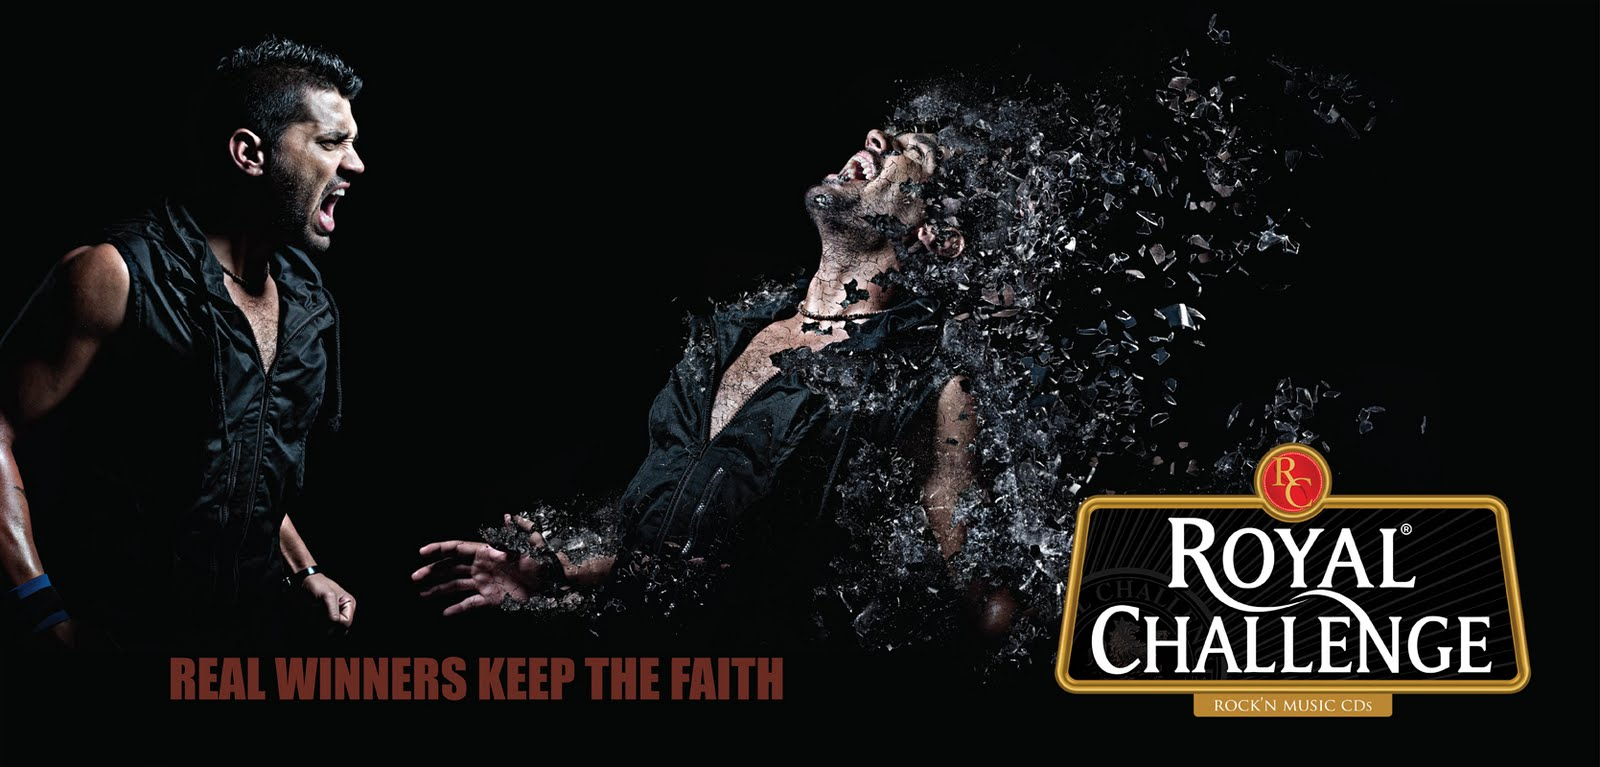
\includegraphics[width=\textwidth]{rcad1.jpg}
\end{figure}

\begin{figure}[h!]
	\caption{Royal Stag Music Advert which would commonly be seen on billboards}
	\centering
		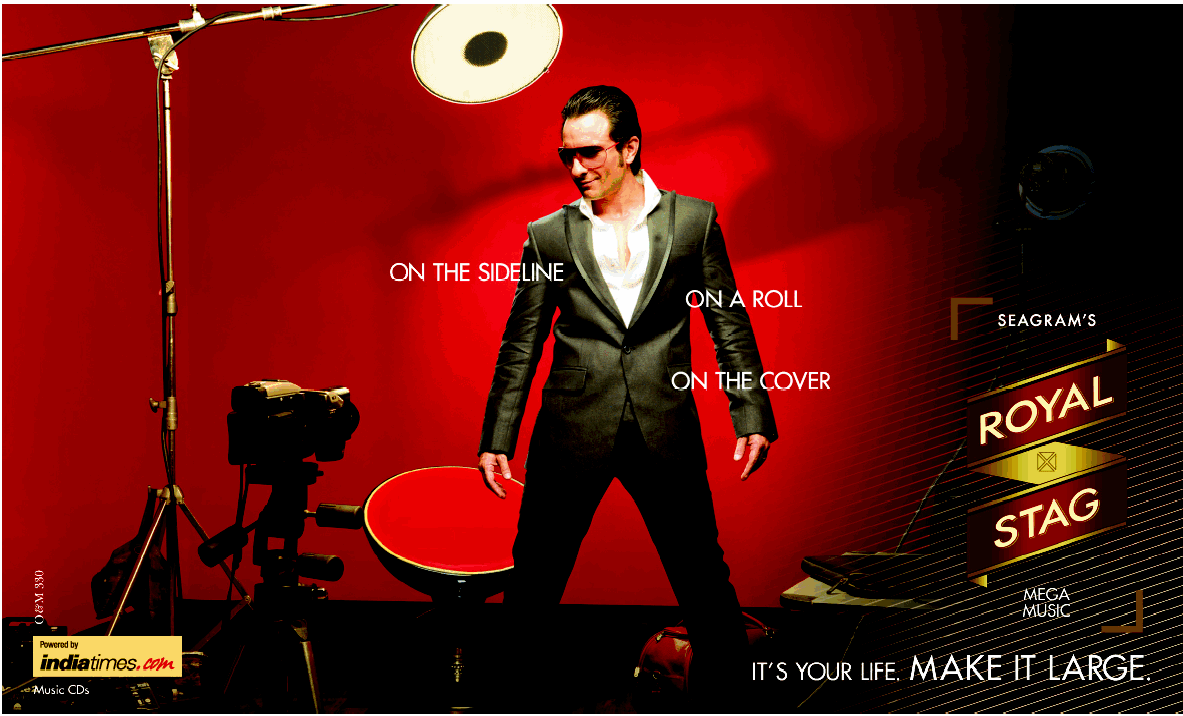
\includegraphics[width=\textwidth]{royalstagad1.png}
\end{figure}

Surveys say that over 80 people out of a 100 understand the actual liquor being
advertised, which means that it is still an effective way of advertising alcohol.

Although currently legal, the government is currently in the process of banning
surrogate advertisements. This is not certain to happen though.

\subsubsection{Alternate Methods of Advertisement}
With the future of surrogate advertising uncertain, some brands have moved to
the event sponsorship and organisation. Examples of this include Kingfisher
sponsoring many teams in the Indian Premier League. Many alcohol brands
have now started sponsoring many glamorous events to spread their name.

\begin{figure}[h!]
	\caption{Royal Stag Music Advert which would commonly be seen on billboards}
	\centering
		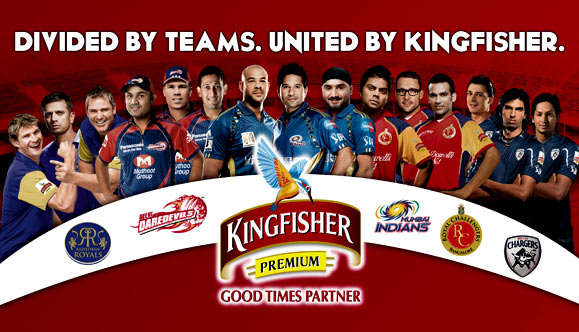
\includegraphics[width=\textwidth]{ipl.jpg}
\end{figure}

\subsection{How We Plan to Advertise Our Product}
\subsubsection{Sponsoring Fashion Shows and Horse Races}
As the microbrewery and cider are new to the city, we would initially have to 
spread the name out by spending big. We believe that the best way to do this is
by sponsoring Fashion Shows and Horse Races, as those are the places where we would
get the maximum number of people we are targetting, who are young people, females
and foreigners.
At the events we sponsor, we would get a limited number of bottles of cider produced
so that the people at these events could taste the cider. There would be large banners
around the location which would advertise the microbrewery. We would also hand out
discount coupons at these events which would encourage people to come to the 
microbrewery. 
\newpage

there is only one other provider of this product hence we see very low competition in this field 

Introducing to bars, clubs and hotels in the major cities in India (Delhi, Mumbai, Goa,
Bangalore, Kolkata). Each city would give a different version of the cider, so we would
get a general idea of what the market prefers taste wise.

Low calorie cider?

Need to make other items with the saame brand name, because advertising is limited. Surrogate advertisement

Affiation with a charity? Provide consumers a "feel good" feeling while buying alcohol.

Corruption free

Use of TV and radio. around a billion people listen to the radio, so sponsor the primetime radio
show to spread the name.

Affiliation with the IPL. International market, so easy to introduce Indians to cider.

Cost based pricing vs Price based costing. Cant do competitive analysis, as no cider exists, but compete with
the local beers, etc. Price based costing wins btw.


 % summary of detailed plan including
	% prioritisation
	% validation
	% offers
	% routes to market

objective - maximise sales -> how

LTV = (Tn + ATV + LT) - (CoA + CoR) 
options which affect LTV

tailor LTV to get maximise value for target customer - guesswork market research
needs to be conducted

how this affects the supply chain
\newpage
\section{Revenue model}
\newpage
\section{Resource, cost and implementation plan}
revenue
 - retail
   licence
   other sales

profit
 - gross
   net
   EBITDA
   NPV

costs
 ...

sources of capital
 % Including headcount plan
\section{Product and systems development plans}
In order to setup a stable and longlasting infrastructure for our business we must take into consideration all the stages and requirements of production. This outlines a coherent development plan as follows.

	\begin{enumerate}
	\item Factory \\
When deciding about our homebase we considered two main criteria. The first regards our situation as a new company without assets. This brought the decision of renting out the factory bulding and equipment. The second criteria regards our main ingrediant requirements. Apples in India are available in the region of Himachal Pradesh. \\

For these reasons we will set our factory near Shimla, capital of Himachal Pradesh and rent the space and equipment necessary for production \\

\textbf{Quantities and Workforce} \\
For our marketing plan we require a relatively small production volume.\\
Workforce availability. \\

\textbf{Quality control}
We must ensure a good quality especially because it is a new product for this market..

	\item Suppliers
		\begin{itemize}
		\item Apple supply \\
			Buy from local farmers %who?
        	Sell residue back to farmers for animals (or agree on lower price)
		\item (Potentially) mango, berries, pares etc. suppliers
		\item Water supply \\
			Divine Waters, Foods Beverages
		\item Sugar supply %who?
		\item Bottling \\
			Home brewers use beer bottles, which work perfectly well, and are inexpensive. This allows the cider to become naturally carbonated.
		\end{itemize}
			
\item Risks \\
Eliminated some risk by:\\
	renting instead of building the factory\\
	buying instead of growing own apples\\
Workforce: lack of experience\\
Collaborators: \\
	\end{enumerate}


%1. how much money do we have
%2. how much can we do without partners
%3. where do we setup factories
%	what gets done in the factory
%4. where do we purchase equipment from
%5. who do we need to work for us
%6. distribution (how?)
\newpage
\section{Capital requirements}
\section{Business opportunities and risks}
\section{Pro-forma financial projections}
\section{Risk analysis}

\end{document}
